\documentclass[oneside]{book}
\usepackage[utf8]{inputenc}
\usepackage{float}
\usepackage{graphicx}
\usepackage{amsmath}
\usepackage{color}
\usepackage{multicol}
\usepackage{ragged2e}
\usepackage{listings}
\usepackage{pdfpages}
\title{Notes de Cours LOG6308}
\date{2017-10-10}
\author{Olivier Sirois}
\setlength\parindent{0pt}
\makeindex
\pagenumbering{arabic}
\begin{document}
\setcounter{page}{1}
\maketitle
\tableofcontents
\chapter{Introduction et Filtres Collaboratifs}
Selon les notes, les recommandations prennent la forme d'un filtre d'information. On essaie de filtrer l'information qu'on ne désire pas avoir. On peut séparer les filtres en deux parties, soit:
\begin{itemize}
\item Filtre passifs: Comme les vidéos et pièces de musique présentées avec le dernier choix fait sur un site, style youtube
\item Filtres Actifs: Comme des courriels de recommandation (se faire envoyer des courriels)
\end{itemize}

On peut définir un système de recommandation comme étant une personnalisation d'interface qui font des choses comme exemples:
\begin{itemize}
\item curation d'articles de presse
\item guide d'étude en fonction des acquis
\item auto-complétion sensible au contete et à l'historique d'utilisation
\end{itemize}

Généralement, la personnalisation à l'utilisateur nécessaite trois types d'information à modéliser et à inférer:
\begin{itemize}
\item Les intérêts et préférences de l'utilisateurs (Présent)
\item Les compétences et connaissances de l'utilisateur (Passé)
\item Les buts de l'utilisateurs (Futur)
\end{itemize}

\subsection{Amazon.com : très efficace!, Intérêts}
Un utilisateur : seulement deux livres d'achetés\\

l'utilisateur à déjà deux livres sur 15 qui sont recommandés, alors c'est quand même pas mal.\\

Dans ces recommandations, plusieurs titres était fort pertinents, soit:\\
\begin{itemize}
\item Machine Learning, Tom Mitchell
\item Categorical Data Analysis, Agresti
\item Data Mining: Practical Machine Learning Tools and Techniques with Java Implementations, Witten \& Frank
\end{itemize}

Plusieurs autres sites tel que Youtube, Itunes, Netflix, WatchOn offres des service similaire.

\subsection{Connaissance}
Certains systèmes essaie de faire des recommandations basé sur les connaissances de certains utilisateurs. Un système comme ALEKS sert à faire des recommandations d'études basé sur les forces et faiblesse de l'utilisateur pour conformer à un certain programme d'étude. Le système pose des question et analyse les réponse de l'utilisateurs et en se basant la dessus, il est capable de déterminer dans quel champ d'étude il devrait travailler dessus pour améliorer sa note.\\

Un système de ce genre donne environ 1 sigma (un écart-type) d'amélioration en moyenne chez les utilisateurs. En moyenne, du tutorat individuel améliore d'environ 2 sigma. Cette marque pourrait être mise comme étant le but de ce genre de systèmes. En moyenne, les systèmes d'aide d'apprentissage aide d'environ 0.3 sigma, ce qui n'est quand même pas négligeable.
\subsection{Intentions et Tâches}
Un exemple de système qui aide à accomplire des tâches de travail est le système de complétion d'Eclipse. En ce mettant en contexte, il faut réaliser que certains des librairies contiennent des classes contenant plus de 381 méthodes. Sa peut être difficile de trouver la méthode qui fait exactement ce que l'on cherche, alors certains systèmes son fait pour analyser ton code, et te faire des recommandations de méthodes basés sur les travails que tu as fait et l'objectifs que tu as. Évidemment, modéliser ce genre de système peut être très complexe et n'est peut-être pas nécessairement souvent correct, mais bon, c'est mieux que rien.\\

Petit rappel que Microsoft à longtemp essayer de faire un système de ce genre  (paperclip). 
\section{Quelques Définition et Taxonomies}
\paragraph{Systèmes de Recommandations et Filtres Collaboratifs}
Ce sont des systèmes qui utilisent des données statistique pour créer et regrouper des utilisateurs selon différentes dimensions (intérêt, navigation, opinions, etc). Une fois regroupé, on détermine les traits et caractéristique communes et déterminantes pour chaque individu groupe afin d'identifier les recommandations pertinentes, c'est-à-dire, des items qui sont bien rater selon les dimensions utiliser dans le groupes d'utilisateur observer.\\

Les recommandations peuvent aussi parfois reposer sur le contenue de ceux-ci (content-based). \\

On peut regrouper les systèmes de recommandations en différentes familles. Comme par exemple:
\begin{itemize}
\item Personnalisation : Des adaptations d'éléments d'interface basé sur un profil personnel
\item Accélérateurs: Des systèmes qui ont pour but d'accélérer certains aspect. Comme par exemple de l'auto-complétion, du pré-chargement(prefetching), de l'auto-correction comme DWIM (Do what I mean)
\item Assistants et Agents: Comme le paperclip de microsoft, Clipper.. Ce sont des systèmes de dialogue qui sont censer aider les gens avec des tâches facile/redondante. Le dialogue coopératif et d'aide est basésur la reconnaissance des intentions et du plan, plus ou moins structuré et prédéterminé, entre un assistant et un assisté

\item Environnement d'apprentissage: Comme vu précédemment, ALEKS, GradeSummit, Lisp Tutor, Andes Tutor. C'est systèmes sont des environnement intelligents d'apprentissage qui utilisent plusieurs approches pour fournir un encadrement à l'apprenant, notamment pour fournir des exercices et capsule d'apprentissage adaptés au besoin d'apprentissage. Pour résumé, ils aident à apprendre et à assimiler la matière.
\end{itemize}

\subsection{Données Utilisées}
Normalement, on se sert de plusieurs sources d'information pour faire nos recommendations. Évidemment, le plus de différentes source d'information qu'on à accès, le plus de liberté et de possibilité que nous pouvons avoir pour faire nos recommandations. Les sources d'informations les plus couramment utilisés sont :
\begin{itemize}
\item Les actions d'utilisateurs:  Simplement prendre en mémoire les actions que les utilisateurs font, de sorte qu'on essaie soit de trouver un pattern, ou d'associer certaines actions avec certains types de recommandations
\item Historique de l'utilisation et de la navigation: Comme par exemple, une matrice utilisateur-visite, qui prend en compte le temps que l'utilisateur prend sur certains items/services. On peut associer avoit une matrice utilisateur-commande, qui prend en compte quel commande l'utilisateur se sert.. 
\item Éléments de contexte: Comme par exemple, la popularité d'un document, la proximité sémantique de termes dans les documents eux-mêmes.. Et aussi, très important, la proximité de profils des différents utilisateurs.
\item Combinaison de données:  utilisation d'une différent combinaison de toutes les sources vues.
\end{itemize}

Pour aller un peu plus en détail, on défini la proximité entre deux utilisateurs comme étant la proximité entre les deux vecteurs représentant ces deux utilisateurs et non la position géographique. On peut utiliser cette même technique avec les documents/URL.\\

d'autre chose dont on peu se servir sont les probabilités. Nous allons les voirs beaucoup plus en détails, mais la probabilité conditionnel est utilisé assez souvent dans la construction des modèles probabiliste. Voir Bayésien.\\

Comme par exemple: On peut définir la probabilité que l'utilisateur clique sur le lien Étudiant actuels de la page d'accueil de Poly(H) étant donnée qu'il a un cooki qui l'idnetifie comme étudiant ($E_1$) et qu'il a accédé à ce lien plus de 5 fois durant les 5 derniers jours($E_2$). \\

\centering
$P(H|E_1,E_2,E_3....E_n)$
\justify

En générale, les actions de l'utilisateurs sont déterminées par les buts que cet utilisateurs veut atteindre. Que sa soit perdre sont temps, ou finir ses notes, l'utilisateur va agir en conséquence. Normalement, un but se décompose en sous-buts et récursivement jusqu'à avoir un ensemble d'actions séquentiel. On peut définir comment un but se transpose en actions par une grammaire récursive ou par un automate fini.\\

\begin{figure}[!ht]
\centering
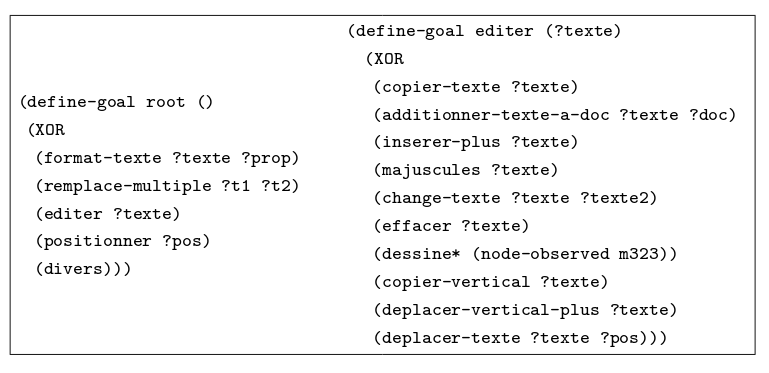
\includegraphics[width = 7cm]{grammaire_recursive.png}
\label{fig:grammaire_recursive}
\caption{Exemple de grammaire recursive.}
\end{figure}

Il y a certaines autres aspects à prendre en considération. Entre autre, les \textbf{facteurs ergonomiques.}
\begin{itemize}
\item Transparence : D'ou vien le rationnel de la recommandation. C'est-à-dire, la logique derrière la recommandation.
\item Crédibilité : La recommandation est-elle fiable ou biaisé ?
\item Contrôle : Est-ce le choix que je ferais si j'avais accès à toutes les options? suis-je pris dans un gettho d'information ? il faut que le système soit capable de bien gérer.
\end{itemize}
\section{item-item et utilisateur-utilisateur}
Le principe d'un filtre collaboratif est de recommander ou filtre l'information pertinente afin de la montrer à l'utilisateur. Comme par exemple:
\begin{itemize}
\item Filtres: Éliminer ou classifier les courriels indésirés; filtrer les nouvelles selon nos intérêts. 
\item Recommandations : suggestion d'achats croisé; publicité personnalisé..
\end{itemize}
l'émerge du web social et les algorithmes de systèmes de recommandations sont de plus en plus répandus. Les utilisations les plus anciennes des filtres collaboratifs remontent jusqu'en 1994 avec l'utilisation du projet GroupLens, qui est un filtre de message pertinents sur UseNet.\\

Aujourd'hui, les grands systèmes de recommandations:
\begin{itemize}
\item Amazon.com: Le plus grand détaillant en ligne, fait un usage intensife de différents types de recommandations
\item Netflix: Recommandation de films/séries, il y a même eux un prix netflix (1M\$). Qui avait pour but d'améliorer les recommandations de film faites par Cinematch et de passer d'un RMSE de 0.96 jusqu'à 0.86 (10\%). Le prix à été lancé en 2066 et gagné en septembre 2009. Deux montréalais ont fait partie de l'équipe gagnantes.\\


\end{itemize} 
\begin{figure}[!ht]
\centering
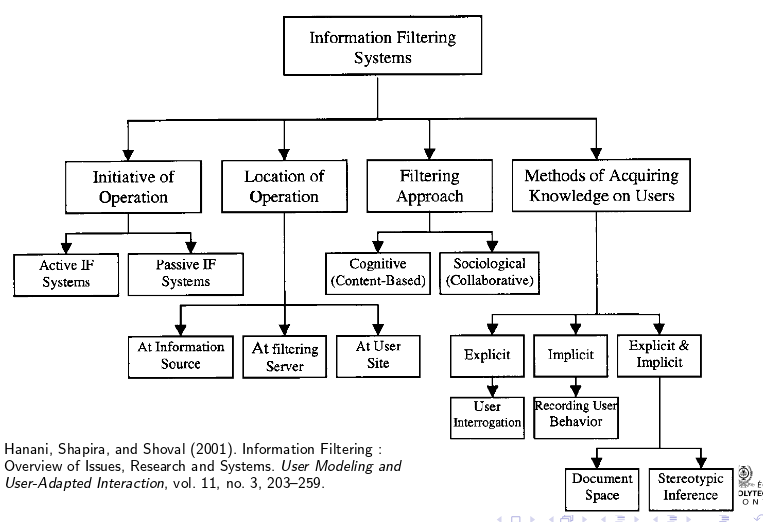
\includegraphics[width = 7cm]{types_systeme_information.png}
\caption{Différents Systèmes d'information}
\label{fig:Systeme_informations}
\end{figure}

Le filtre d'informations peut soit être passif ou actif.
\paragraph{Système Passif} Cherche à réduire le flot d'information, comme par exemple un filtre polluriel. (Cherche à éliminer du mauvais)
\paragraph{Système Actif} Cherche à créer un flot d'information en extrayant de l'information de différentes sources pour les livrés à l'utilisation. (Cherche à ajouter du bon)\\

Le filtre se trouve généralement à trois endroits différents:
\begin{itemize}
\item Au poste de travail (client side)
\item À la source d'information (Server Side)
\item sur un serveur de filtre dédier
\end{itemize}

Un filtre passif est généralement situé sur le poste client étant donné qu'il ne cherche qu'à enlever de l'information. Par contre, un filtre actif sera normalement mit sur la source ou sur un serveur de filtre étant le grand nombre de données dont il doit processer pour pouvoir effectuer sa recommandation.\\

De plus, on peut spécifier aussi la méthodes d'acquisition de l'information sur l'utilisateur dans notre filtre. Normalement, on utilise des méthodes:
\begin{itemize}
\item Explicite: l'utilisateur spécifie ses préférences (généralement pas utiliser étant donné que ces méthodes sont très aggressives et peuvent tanner l'utilisateur)
\item Implicite: les préférences sont déduites du comportement de l'utilisateur
\item Combinaison: l'utilisateur spécifie quelques paramêtre de préférences mais un traitement est réalisé pour établir des informations implicites en même temps.
\end{itemize}

Normalement, l'approche \textbf{collaborative} du filtrage se base sur des facteurs sociologiques explicite et implicite. Comme par exemple, on utilise les votes (explicite) ainsi que des données d'achat et de consultations de pages (implicite) pour établire des similarités entre les différents utilisateur. Par contre, l'approche collaborative peut être utiliser de différentes manière. Comme par exemple, sa peut être utiliser en comparant les items et établir des utilisateur recommandés ou comparés des utilisateur et recommandés des items. 
\subsection{utilisateurs-utilisateurs}
On essaie de classifier les gens selon leur intérêts, leurs votes, leur comportements ou toute autre dimensions qu'on juge pertinentes. On effectue des recommandations basées sur le groupes le plus près et le plus représentatif d'un individu. On recommandera ainsi un élément très caractéristique du groupe qui n'est pas dans le profil de l'individu
\subsection{items-items}
On essaie rechercher des items qui ont des profils d'intérêts similaires. On fait une recommandation en fonction de l'item affiché ou d'un historique d'items (on prend les items achetés/bien rater, on regarde les items les plus près selon certaines dimensions et on effectue une recommandation basé sur ce groupe.) 

\paragraph{Approche Contenue}
Une approche différente, elle cherche à analyser les propriétés des items au lieu des différentes dimensions sociologique de l'approche collaborative (votes, temps passer). Mais cherche toujours les similarités entre les items.
\section{Approche Mémoire vs Approche Modèle}
On différencie aussi les différents algorithme de systèmes de recommandations en fonction de la gestion de la mémoire. On différencie les algorithme comme étant:
\begin{itemize}
\item Memory-Based (basé mémoire): On effectue une recherche dans une Base de Données et on l'utilise certains algorithme avec des quantités massive d'informations pour effectuer nos recommandations
\item Model-Based (basé model): C'est basé sur l'apprentissage d'un model. On utilise une base de données pour entraîner un model qui ensuite permet la prédiction de l'item pertinent sans avoir à faire une série de calcule intensif. Par contre, il faut prendre en considération que sa peut être long entraîner un model.
\end{itemize}

\section{Algorithme Utilisateur-Utilisateur et Items-Items}

En regroupant l'information récolté de nos méthodes implicites et explicites, on peut finalement les représentées sous formes d'une matrice:\\

\begin{figure}[!ht]
\centering
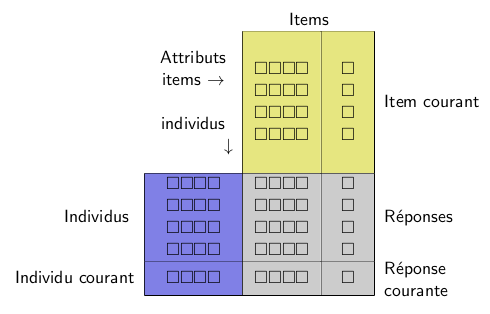
\includegraphics[width = 7cm]{matrice_features.png}
\caption{représentation de nos features dans une grande matrice}
\label{fig:matrice_features}
\end{figure}

On condense donc l'information des utilisateurs et des items dans une seul grande structure de données. Par contre, ce qui nous intéresse c'est le millieu de cette matrice ou on voit les liens entre nos utilisateurs et nos produits. C'est en faisant des opérations sur ces liens que nous allons pouvoir faire nos recommandations. Commençons premièrement par faire une recommandation en se basant sur les différents profils de nos utilisateurs.

\subsection{Utilisateurs-Utilisateur}
Prenons comme exemple initiales cette matrice contenant des votes de 4 utilisateurs pour 4 items différents.
\begin{figure}[!ht]
\centering
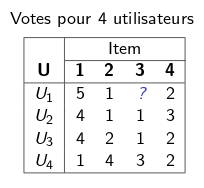
\includegraphics[width=7cm]{exemple_user_user.png}
\caption{notre matrice pour les 4 utilisateurs et 4 items}
\label{fig:ex_user_user}
\end{figure}

Notre objectif est de prédire les votes d'un utilisateur spécifique à partir de notre Base de Données des autres votes des utilisateurs.\\

La valeur estimé de l'utilisateur a pour un item j, $E(v_{a,j})$ est la somme pondéré des votes des autes utilisateurs $v_i$ qui ont des votes communs, soit:\\

\centering
$E(v_{a,j})$ = $\bar{v}_a + k \sum\limits_i^n w_{a,i}(v_{i,j} - \bar{v}_i)$
\justify

Ou a est notre utilisateur, j est notre item cibler et i est l'ensemble de tous les autres items.\\

Le poids w dans la formule peut représenter plusieurs chose, elle peut par exemple représenter une corrélation, une distance euclidienne, un coéfficient de similarité quelconque défini par le système. la constante k est une normalisation des poids à un, qui peut être représenter par :\\

\centering
$k = \frac{1}{\sum\limits_i |w_{a,i}|}$
\justify

\subsubsection{Corrélation Pearson}
Une estimation de poids très populaire est celle de la corrélation pearson. la corrélation Pearson est une mesure statistqiue très commune qui à originalement été utilisé pour les filtres collaboratifs par le projet GroupLens (Resnick et al. 1994). La corrélation entre les \textbf{utilisateurs} a et i est : \\

\centering
$w_{cor(a,i} = 
\frac{cov(a,i)}
{\sigma_a \sigma_i} =
\frac
{\sum\limits_j (v_{a,j} - \bar{v}_a )( v_{i,j} - \bar{v}_i)}
{\sqrt{\sum\limits_j (v_{a,j} - \bar{v}_a ) ^2 \sum\limits_j ( v_{i,j} - \bar{v}_i)^2}}$
\justify

Pour l'exemple d'en haut, ces calculs reviennent au résultats suivant:

\begin{figure}[!ht]
\centering
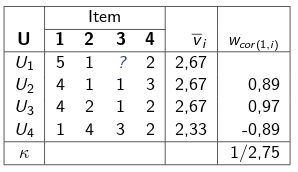
\includegraphics[width = 7cm]{resultats_user_user.png}
\caption{Résultats des calculs pour la réponse utilisateur-utilisateur}
\label{fig:rep_user_user}
\end{figure}
Ce qui nous donne une réponse de 1.34 pour $E(v_{1,3})$\\

voici la démarche:\\

\begin{figure}[!ht]
\centering
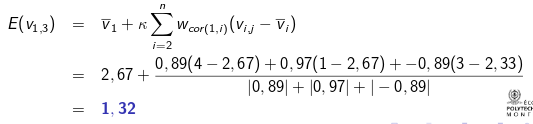
\includegraphics[width=7cm]{demarche_user_user.png}
\caption{Démarche pour utilisateur utilisateur}
\label{fig:demarche_user_user}
\end{figure}

On peut refaire cette même série de calcul mais au lieu d'utiliser la corrélation Pearson on pourrait utiliser la mesure du cosinus. Cela nous permet d'avoir de meilleurs résultats quand nous données tendent vers 0.\\

\centering
$w_{cos(1,i)} =
\frac
{\sum\limits_j v_{1,j} v_{i,j}}
{\sqrt{\sum\limits_{k\in l_1} v_{1,k}^2 \sum\limits_{k\in l_i} v_{i,k}^2}}$\\


$ = \frac{v_i v_i}{\parallel v_1 \parallel \parallel v_i \parallel}$\\

\justify
Chaque utilisateur représente ainsi un vecteur dans un espace de vote et on cherche celui qui a le vecteur le plus près (parallèle). Cette différente méthode, avec la mesure du cosinus, va nous donner les résultats suivant:\\

\begin{figure}[!ht]
\centering
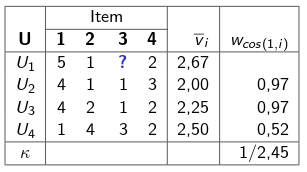
\includegraphics[width=7cm]{resultats_cosinus.png}
\caption{résultats du cosinus}
\label{fig:resultats_cosinus}
\end{figure}

Le résultats de ces calculs nous donnent un résultats de 1.49 . ce qui en quand même vraiment différent. \\


\subsection{K nearest Neighbour}
Le principe est qu'on utilise le vote moyen, ou pondéré, des n utilisateurs le splus rapprochés dans l'espace vectoriel des votes. La distance euclidienne est généralement utilisé pour cette fin:\\

\centering
$d(a,i) = \sqrt{\sum\limits_j (v_{a,j} - \bar{v}_{i,j})^2}$
\justify

Pour chaque item j, on calcule la racin carrée de la somme des carrés des différences entre les votes des utilisateurs a et i. Les utilisateur les plus proches voisins sont ceux ayant les premières n valeurs. On fais un rankings des utilisateur les plus près de notre utilisateurs ciblé. On détermine alors la valeur du vote de l'utilisateur a par la moyenne, potentiellement pondérée, de ces utilisateurs. Comme on peut voir dans l'exemple ci-dessous, les deux utilisateurs les plus prochs de $U_1$ sont $U_2$ et $U_3$. Leurs distance avec $U_1$ est de $\sqrt{2}$. En ne conservsant que ces deux plus proches voisin, la réponse est de $E(v)_{1,3} = 1.0$, ce qui n'est pas très précis..

\begin{figure}[!ht]
\centering
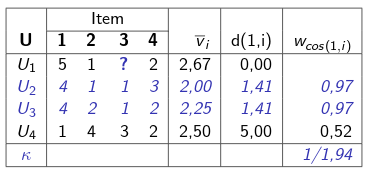
\includegraphics[width = 7cm]{knn.png}
\caption{exemple K nearest Neighbour}
\label{fig:knn_exemple}
\end{figure}

On peut continuer notre analyse. La valeur d'une corrélation ou d'un cosinus basée sur un plus grand nombre de votes commun devrait avoir un poids plus important qu'un valeur basée sur un plus petit nombre. Il est donc fréquent de faire la correction suivante au poids $w_{u,v}$ : \\

\centering
$w'_{u,v} = \frac{max(v_{u,v}, \gamma}{\gamma} * w_{u,v}$
\justify
Ou $v_{u,v}$ est le nombre de votes communs entre les utilisateur u et v et ou gamma est un constante représentant le nombre minimum de votes pour effectuer cette correction, par exemple, Herlocker et coll(1999) utilisent gamma  = 5.
\subsection{item-item}
Les algorithme précédent cherchent des similarités entre utilisateur pour ensuite proposer les items les plus populaires des utilisateur voisins, notamment par une some pondérée similarité-utilisatuer par item pour suggérer les items (équations 1). \\

L'approche item-item cherche plutôt des similarité entre les items. Dès qu'un utilisateur s'intéresse à un item, on lui suggère des items similaires. \\

Les similarités dans ce cas ci peuvent être estimés par le cosinus ou la corrélation entre des items, sauf qu'on transpose la matrice pour faire le calcule de la similarité item-item plutôt qu'utilisateur-utilisateur.\\

finalement, on procède de façon analogue, à l'approche utilisateur-utilisateur en utilisant une somme pondéré.\\

comparément à l'algorithme utilisateur-utilisateur, l'item-item utilise la même méthode, mais au lieu de l'appliquer sur des vecteur d'utilisateur on l'applique sur des vecteurs d'items. \\

\begin{figure}[!ht]
\centering
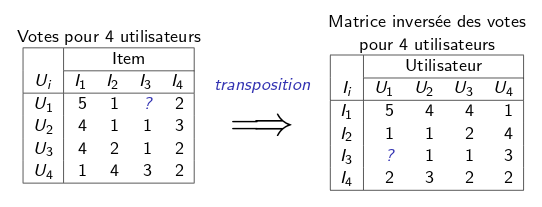
\includegraphics[width = 7cm]{item_item.png}
\caption{transposition de la matrice pour l'item-item}
\label{fig:item_item_transpose}
\end{figure}

En ne gardant que les items 2 et 4 comme plus proche voisins. On peut déduire la réponse suivante à partir de cette question.
\begin{figure}[!ht]
\centering
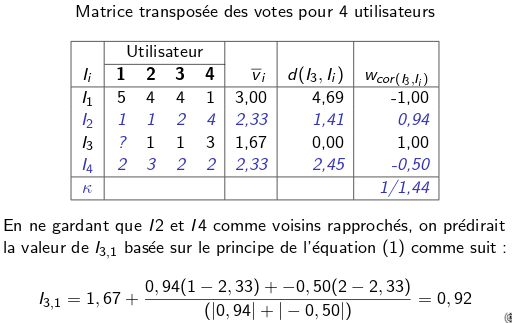
\includegraphics[width = 7cm]{probleme_item_item.png}
\caption{probleme items items}
\label{fig:probleme_item_item}
\end{figure}

On peut faire les mêmes calculs qu'à l'exemple précédent mais en utilisant le cosinus comme poids. Par contre, on obtiendrait un résultat de .78 ce qui n'est pas exactement très bon. En utilisant le cosinus normalisé, on pourrait vraiment avoir une mesure beaucoup plus précise. Pour faire sa, nous avons qu'a soustraire la moyenne des rating par utilisateur dans le calcul du poids du cosinus dans le cas d'un calcul item-item (soustraire rating par item dans le cas utilisateur=utilisateur??). Ce qui nous donnerait maintenant un résultats de 1.62, ce qui est beaucoup mieux. \\

Pour résumer, c'est bien de normaliser en fonction de ce qu'on compare pour prendre en compte des différences de votages, comme par exemple un utilisateur qui vote très haut comparément à un utilisateur qui vote très bas. (genre une moyenne de vote de 4 versus un moyenne de vote de 1).\\

Maintenant, ce qui nous intéresse de la méthode item-item c'est de faire une recommendation d'item à un utilisateur en utilisant des items similaire à ceux dont l'utilisateur s'intéresse. Maintenant supposons un item d'intérêt i pour l'utilisateur u, un approche possible serait
\begin{itemize}
\item Trouver les N items le splus similaires à i
\item De ces N items, choisir les R items dont on calcule le vote le plus élevé pour u.
\end{itemize}

\section{TF-IDF}
On peut utiliser la transformation TF-IDF pour la recherche d'information. On peut conclure que la similarité de votes pour un item comportant un grand nombre de votes n'a pas le même poids qu'un vote similaire pour un item comportant très peu de votes. Comme par exemple, Vu que StarWars à beaucoup de bons vote de tout le monde. Sa veut dire que les gens vont naturellement trouver le film bon, alors le recommander n'a pas un impact très intense. Par contre, un film ayant peut de vote mais qui est quand même bien rater pour un utilisateur serait un bien meilleur choix de recommandation. \\

On utilise la transformation TF-IDF pour prendre en compte ces différences:\\

Pour l'item j, son poid $w_j$ et son nouveau poids pondéré, $w'_j$\\

\centering
$w'_j = w_j log(\frac{n}{n_j})$\\
\justify

Ou n est le nombre total d'individus et $n_j$ est le nombre d'invidus qui ont exprimé un vote pour l'item spécifier. 

\section{Mesure de Performance}
Pour mesurer la performance de nos algorithe, on mesure normalement l'erreur entre la valeur prédit et la valeur réelle. La manière dont on mesure l'erreur peut varier, on peut utiliser l'erreur au carré, l'erreur absolue, la racine de l'erreur au carré, c'est très flexible. \\

La moyenne des erreurs au carré ou plus communément, l'erreur quadratique:\\
\centering
$\sqrt{\frac{\sum\limits_i^N (\bar{x}_i - x_i)^2}{N}}$\\
\justify

ou par exemple l'erreur absolue moyenne:\\

\centering
$\frac{\sum\limits_i^N |(\bar{x}_i - x_i)|}{N}$
\justify

Une autre mesure très utile est d'utiliser le \textbf{Receiver operator Characteristic}. Entre autre, c'est de mesure le taux de vrais positif versus faux positif, vrais négatifs versus faux négatif. Vice versa. On mesure l'évolution du taux en fonction de notre algorithme.

\begin{figure}[!ht]
\centering
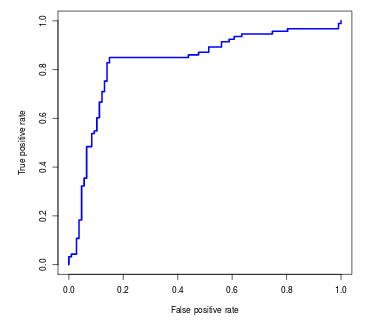
\includegraphics[width = 7cm]{ROC.png}
\caption{Receiver Operator Characteristic}
\label{fig:ROC}
\end{figure}

On essaie normalement de maximiser l'aire sous la courbe, ou : \textbf{AUC, Area Under the Curve}\\

Lors de simulations, on utilise la validation croisé. Le principe de la validation croisée est de séparé nos donnée en un ensemble d'entraînement et un ensemble de validation (de test). Ce qu'on fait:
\begin{itemize}
\item On retire des données de notre ensemble de données original, et on les conserve pour des tests
\item On cible les valeurs qu'on à enlever et on prédit les votes avec notre algorithme
\item On compare les votes qu'on à prédit avec les vrais votes qu'on à sauver
\end{itemize}

Étant donnée la stochasticité de cette méthode, on essaie généralement de répéter l'expérience plusieurs fois en raison de l'impact que l'enlevement de certaines données peuvent avoir sur le calculs des votes prédits. On peut aussi faire des variations sur notre méthode de séparé nos données. Comme par exemple, on peut seulement en enlever une, tester, la remettre, en enlever une autre, tester, etc.\\

Aux fins de comparaison, on élimine du bloc de validation et d'entraînement de l'individu cible, et on rapporte ensuite le score moyens. 

\chapter{Méthode contenue, PageRank et un peu de Bayésien}
Les méthode collaborative utilisent des mesures directe et indirecte de l'\textbf{intérêt} pour mesure des similarités entre des utilisateurs/items/peu importe. Cependant, les approche contenus utilisent des attributs de ces objets et utilisateur pour les comparés. On utilise communément la \textbf{sémantique} \textbf{démograhique} ou autre attributs associés aux items ou aux utilisateurs afin d'établir la similarité. Les approche contenus ont plusieurs d'affinités avec les technique de recherche d'informations.\\

Normalemnt, les approches items-items et utilisateurs-utilisateurs sont dites \textbf{basés mémoire}. Leur ordre de complexités est de l'ordre de $O(mn^2)$ ou n est le nombre d'utilisateur et m le nombre d'items. (pour l'approche item-item, l'inverse pour u-u). Pour des applications ou le temps de réponse est critique et ou la Base de Données est grande, le calcul basé mémoire doit s'effectuer au préalable et le résultat stocké en mémoire pour une consultation rapide. Par contre, si l'information change souvent, ce qui est le cas généralement pour les utilisateur ayant peu d'historique, l'approche n'est pas très idéale. C'est pourquoi une approche \textbf{basé modèle}, peut être une bien meilleur idée. Le modèle probabiliste est un très bon candidats.

\begin{figure}[!ht]
\centering
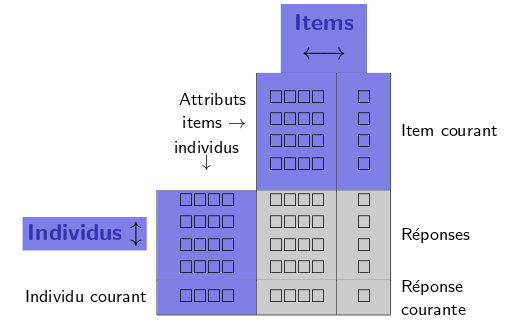
\includegraphics[width = 7cm]{contenu.png}
\caption{Approche contenu}
\label{fig:contenu}
\end{figure}

\section{Modèles Probabiliste}
Le principe d'un modèle probabiliste est d'utiliser des facteurs propres aux items et/ou aux utilisateurs. Soit:
\begin{itemize}
\item utilisateurs:
\begin{itemize}
\item âge
\item profession
\item sexe
\item code postal (position géogrpahique)
\item etc.
\end{itemize}
\item items
\begin{itemize}
\item auteur
\item mots-clés
\item année de production
\item etc.
\end{itemize}
\end{itemize}

Quand notre base de données est assez grande, certains items s'addressent à des populations spécifiques et ils sont reconnaissables par leur attributs de contenu. Les votes les plus probable peuvent s'exprimer sous la forme de \textbf{probabilité conditionnelle}. qui veut dire, la probabilité du vote v étant donnée les attribut utilisateur et items:\\

\centering
$P(v_{ij} = x | A_{ik} = 'ing') = \frac{P(v_{ij} = x, A_{ik} = 'ing')}{P(A_{ik} = 'ing')}$
\justify

ou par exemple, le film $v_{ij}$ est le vote pour le film j de l'utilisateur i et $A_{ik}$ est l'attribut profession de l'utilisateur i. 
\subsection{Correction de Laplace}
Pour ces calculs, on peut aussi rajouter la base de ratio de fréquence. Car lorsque notre base de donnée est très petite, nos ratios peuvent données des résultats un peu étrange, on utilisera donc la \textbf{correction de Laplace} pour pouvoir corriger ces inégalités..\\

\centering
$\frac{x_1 + 1}{(x_1 + x_2) + 2}$\\
\justify

Cette correction intègre une notion de probabilité antérieur et évite les biaise des petits échantillons de même que les ratios singulier de 1/1, 0/1, 0/0. 

\subsection{Exemple}
Maintenant, supposons le vote d'un homme ingénieur:\\

\centering
$P(v_{ij} = x | A_{ik1} = 'ing', A_{ik2} = 'H') = 
\frac
{P(v_{ij} = x, A_{ik1} = 'ing', A_{ik2} = 'H')}
{P(A_{ik1} = 'ing', A_{ik2} = 'H')}$
\justify

Le problème avec ce calcul est que la combinaison de facteurs divise les fréquences à chaque facteur que l'on rajoute. On peut rapidement trouver avec aucun cas. \textbf{Solution}: On postule l'indépendance des facteurs\\

\centering
$P(v_{ij}|A_{ik1}, A_{ik2}) = P(v_{ij})P(A_{ik1}|v_{ij})P(A_{ik2}|v_{ij})$
\justify

de manière générale..\\

\centering
$P(C|F_1,...,F_n) = \frac{1}{Z} * p(C) \prod\limits_{i=1}^n p(F_i|C)$
\justify
ou C est une classe et F sont des attributs. Z est une valeur qui ne dépend pas de C, de sorte que lorsqu'il s'agit d'estimer la class la plus probable, on peut l'ignorer.\\

\section{Autres Approches probabiliste}
Plusieurs modèles ont ét proposé pour fournir un estimation probabiliste des votes. Par exemple, on peut utiliser l'espérance en fonctions des items pour estimer le votes d'un utilisateur. \\

La valeur attendue d'un vote (sur une échelle ordonnée) est la somme pondérée de la probabilité de chaque valeur par sa probabilité:\\

\centering
$E(v) = \sum\limits_i P(v=i)i$
\justify

La formulation de cette équation dans le contexte d'esitmer le vote de l'utilisateur actif, a pour un itemj est :\\

\centering
$E(v_{a,j}) = \sum\limits_i P(v_{a,j} = i|v_{a,k},k \in I_a)i$
\justify

c-à-d. que $E(v_{a,j})$ est la somme pondérée des probabilités de chaque vote étant donnée les votes aux autes items pour l'utilisateur actif. 

\section{Modèle Par Classe (Clustering)}
Une première approche repose sur la définition de classe d'utilisateur. Ces classes sont définies en fonction de leur capacité à disciminer les préférences entre les utilisateurs.\\

\centering
$(P(C=c|v_1,....v_n) = P(C=c)\prod_i P(v_i|C=c)$\\
\justify

Ensuite, on calcule les probabilités qu'un utilisateur appartienne à chaque classe respective à la lumière de ses votes et on utilise ses probabilité dans l'équation (1). Cette approche nécessaite le recours à l'algorithme EM pour obtenir probablités et de déterminer un nombre adéquat de classes par des techniques d'exploration statistique. \\

Une autre approche probabiliste serait de dériver des probabilités conditionelle entre les noeuds eux-mêmes. Breese et Coll. utilisent par exemple un arbre de décision comme celui ci-dessous. Les noeuds terminaux représentent la probabilité de visionner 'Melrose Place' conditionnellement à avoir visionné les noeuds parents.\\

\begin{figure}[!ht]
\centering
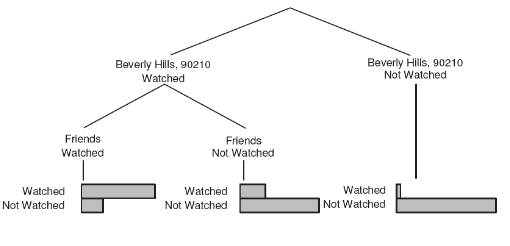
\includegraphics[width = 7cm]{decision_tree.png}
\caption{Melrose Place}
\label{fig:decision_tree}
\end{figure}

Aussi, plutot que de faire un arbre de décision, on pourrait aussi faire un calcul de probabilité postérieur:\\

\centering
$P(v_i|v_j\in S) = \prod\limits_{j\in S} P(v_j|v_i)$
\justify

Il faut faire une sélection de noeuds pertinents, $v_j \in S$, puis établir les valeurs de $P(v_j|v_i)$ à partir des données.\\

Un test d'indépendance entre $v_i$ et tous les autres noeuds permet d'effectuer une première sélection de facon simple. Cette approche est semblable aux réseaux bayésien, à la différence qu'on ne crée que des réseaux bayésiens dits naïfs.\\

Les calculs reposent sur un hypothèse d'indépendance des votes étant donnée l'appartenance à une classe, ou l'indépendance conditionnelle des votes entre eux. Dans le cas de l'approche des classes, le calcul nécessite un entraînement avec des données et repose sur 
\begin{itemize}
\item un algorithme pour définir les classes optimales
\item estimer les paramêtre du modèle. qui peut être assez difficile.
\end{itemize}

On peut aussi utiliser une approche graphiques, Ces approches indique les interdépendance entre les votes et les items pour inférer la probabilité d'un vote à un item donné. Breese et Al. propose une approche basées sur les modèles bayésiens tandis que Heckerman et al. suggèrent un approche basé sur un modèle de réseaux de dépendance. Les deux approche sont comparables en termes d'acuité et performance de 2\% à 4 \% mieux que les méthodes d'espace vectoriels dans les expériences rapportés.L’approche de
réseaux de dépendance est cependant moins gourmande en
ressources mémoire et de calcul.
\section{Arbre de décision}
\begin{itemize}
\item Avantages:
\begin{itemize}
\item Ces modèls sont plus précis pour prédire les votes
\item Plus rapides dans la mesure ou l'on peut créer un modèle avec des paramête plutot que de prendre une approche ou l'on doit faire des calculs basés sur l'ensemble des données
\end{itemize}
\item Désavantages
\begin{itemize}
\item Déploiement beaucoup plus complexes
\item Nécessite une maîtrise des techniues de modélisation bayésienne et d'estimation de paramêtre relativement sophistiqué
\end{itemize}
\end{itemize}

Comme discutés précédemment, il est aussi possible d'utiliser la fréquence inverse des votes pour pouvoir donnée plus de poids aux votes moins fréquents en modulant le poids par l'équivalent de la fréquence inverse des documents (TF-IDF)\\

Une seconde transformation du vote consisterait à pénaliser les votes qui sont plus faible pour compenser le fait que les utilisateurs ont moins tendance à votes pouer les items qu'ils n'aiment pas.

\subsection{Breese et Coll.}
\begin{figure}[!ht]
\centering
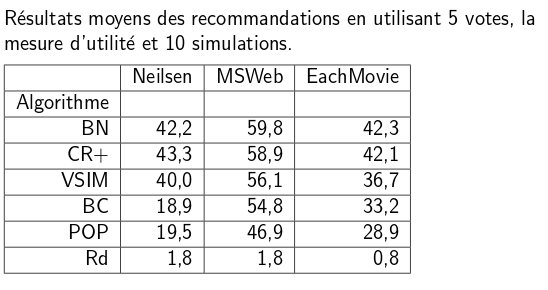
\includegraphics[width = 7cm]{breese.png}
\caption{Résultats de l'expérience breese et col.}
\label{fig:breese}
\end{figure}

l'utilisation de la fréquence inverse utilisateur améliore les résultats mais de façon variable. On peut voir une amélioration de 1 à 3 \% pour la corrélation et le cosinus pour la prédiction de recommandations. et de 3 à 25 \% pour la prédiction d'un vote individuel, plus grande amélioration pour le cosinus que la corrélation, par contre, sa ne s'applique qu'aux données EachMovie.\\

l'amplification du score améliore aussi les résultats de 1 à 10\% mais surtout pour les données de télévision et très peu pour EachMovie.\\

La taille du corpus d'entraînement influence quand même grandement la performance jusqu'à atteindre un seuil maximale (convergence).\\

\begin{figure}[!ht]
\centering
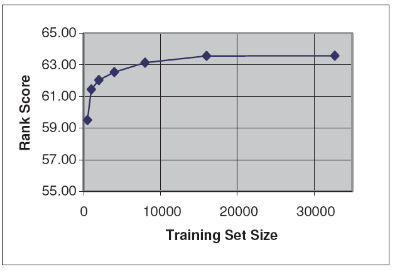
\includegraphics[width = 7cm]{corpus.png}
\caption{corpus d'entraînement pour breese et col.}
\label{fig:corpus}
\end{figure}


\section{PageRank (Popularité)}
Par définition, les items plus populaire intéressent plus d'invidivus. Cependant, c'est quand même difficile de représenter la popularité d'un document en fonction d'un nombre et de pouvoir le comparé avec un autres. Par contre, à l'aide de liens entre les documents, on peut mesurés la popularité d'un document à l'aide des liens entre eux. Les références dans le cas du web sont les liens entres les différents pages. \\

l'algorithme PageRank, définit par Larry Page dans le début des années de google. est particulièrement bien adapté à la mesure de popularité. Le principe est d'avoir une requète dans un monde W, qui retourne une ensemble de page s correspondant à la requète ciblé, soit par mots-clés, distance euclidienne à partir d'une référence, etc. On peut aussi définir s' comme étant les pages référencés par les pages dans notre domaine initiale s. Selon l'algorithme Pagerank, dans notre figure, (b) serait la page la plus pertinente car elle est la plus référencés de s. Cependant, en faisant l'extension du domaine à s', on peut voir que la page (a) est bien meilleur. Il existe plusieurs variante possible selon qu'on différencie entre les types de liens ou qu'on ne tien compte que de s et s' par exemple. En plus, la définition de s et s' est complètement au choix de l'architecte du système.\\

l'algorithme de base de PageRank est la suivante:\\

\centering
$PageRank(A) = (1-d) + d \sum\limits_{D1...Dn} \frac{PageRank(D_i)}{C(D_i)}$\\
\justify
Ou:
\begin{itemize}
\item $D_n$ sont les page qui réfèrent à A (liens entrant)
\item $C(D_i)$ est le nombre de référencs de la page i (les liens sortants)
\item d est un faceur d'ajustement dans l'intervalle [0,1], notamment pour permettre aux pages sans liens entrants d'avoir une cote et pour faciliter la convergence pour les calculs des pages référencés par de telles page. Une valeur de base pourrait ête de 0.85
\end{itemize}
Cet algorithme est itératif et les valeurs convergent après quelques itérations (souvent en dessous de 10). On peut initialiser les PageRank et ajouter 1 à C(D) pour éviter des division par 0.\\

Le modèle calcule la probabilité que l'on accède à une page en suivant les liens de façons aléatoire. Le facteur d'atténuation d représente la probabilité qu'un individu continu d'accéder à des pages; donc (1-d) est la probabilité qu'il arrête. \\

Pour que la somme des PageRank donne 1, on divise le facteur d'atténuation par N, le nombre total de pages:\\

\centering
$PageRank(A) = \frac{(1-d)}{N} + d \sum\limits_{D1...Dn} \frac{PageRank(D_i)}{C(D_i)}$\\
\justify

Si on considère le réseau de liens comme un chaîne de Markov ou les pages sont des états, le PageRank représente en fait la probabilité qu'un individu soit sur une page donnée par une navigation aléatoire. 

\subsection{Calcul de manière vectoriel}
Pour faire le calcul de manière vectoriel, voici la meilleur manière de calculer le Pagerank:\\

soit:
\begin{itemize}
\item r: vecteur des valeurs de Pagerank (initialiser à 1)
\item s:vecteur du nombre de liens sortant
\item A: matrice d'adjacances (les références)
\item \textit{d}: le facteur d'amortissement
\item \textbf{d}: un vecteur d'amortissement de longueur n contenant
\item n: le nombre de document
\end{itemize}
La valeur de R, qui est le page de chaque articles, serait calculer de la manière suivante:\\

\centering
$r = \frac{(1-d)}{n} + dA(\frac{r}{s}$
\justify
 
 
\subsection{Exemple}
En supposant une valeur d de 0.85, et en initialisant le PR de chaque page à 1, les valeurs des PR à chaque itération sont alors:

\begin{figure}[!ht]
\centering
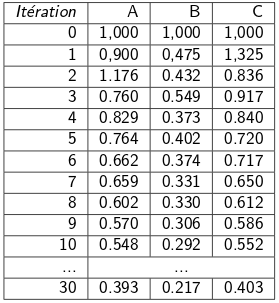
\includegraphics[width = 7cm]{pagerank_scores.png}
\caption{Valeurs de PageRank pour chaque itérations de notre graphe ci-dessous}
\label{fig:valeurs_pagerank_iterations}
\end{figure}

\begin{figure}[!ht]
\centering
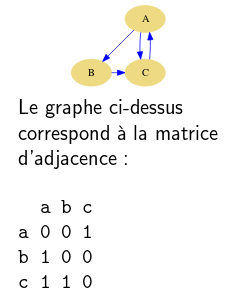
\includegraphics[width = 7cm]{matrice_adjacance.png}
\caption{Notre matrice d'adjacance avec graphe}
\label{fig:matrice_adjacance}
\end{figure}

l'algorithme PageRank à révolutionner la recherche d'information sur le web, un des raisons pourrait être expliquer en raison du fait que Pagerank chercher à vraiment modéliser l'interactions entres les différents articles en fonctions de comment les articles interagissent entres-elles. Sa fait en sorte qu'on exprime d'une manière beaucoup plus intime les relations entre les différents articles. C'est pourquoi l'approche Pagerank est très performante et peut rivaliser les approches d'espaces vectorielles et proabiliste.\\

l'algorithme Pagerank peut être utiliser pour recommander des articles. Premièrement, on peut cibler un article spécifique sur lequel on veut trouver des articles voisins et faire des recommandations d'article qui ressemble à cet article cibler. On peut faire sa en spécifiant un domaine S qui prendrait toutes les articles auquel l'article en question fait références. On calculerait ensuite le PageRank pour toute ces articles, et ensuite on prendrait les articles ayant les indices Pagerank les plus haut afin de les recommandés.\\

\subsection{Puissance des Matrices}
Un aspect très intéressant est la relation entre les différentes puissance des matrice d'adjacance. en représentant un graphe sous la forme d'une matrice d'adjacance (ou de transisiton). Il est possible de déterminer les chemins transitifs entre les noeuds par la puissance de la matrice. ainsi, supposons un matrice de transition M entre quatre noeuds (a,b,c,d) et ou (i,j) = 1 indique l'existence d'un lien i $\rightarrow$ j, les graphiques peuvent être représenter comme ceux-ci, avec les valeurs de matrice de a à c étant de deux pour la deuxième, qui compte les liens entre c et a:\\

\begin{figure}
\centering
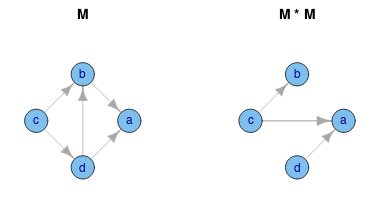
\includegraphics[width = 7cm]{transition.png}
\caption{Démonstration d'une deuxième puissance d'une matrice de transition/adjacance}
\label{fig:transition}
\end{figure}

\section{Rappel Théorie Bayésienne}

Voir section des notes d'INF8215

\chapter{Réduction de Dimensions}
Normalement, nos systèmes essaie de faire une recommandations basé sur une multitude de films (1000+). Quoique précise, ces recommandations nécessite un nombre assez élevés de cycles CPU pour calculer. Une des méthodes que l'on propose pour réduire l'intensité des calculs est d'effectuer une réduction de dimension pour nos données.\\
\section{Intuition}
Le principe/intuition derrière la réduction de dimensions est de 'séparé' les films selon certaines dimensions. Par exemple, on peut regrouper les films comme étant des films d'horreur, des films d'actions, des films romantique.. etc. Par contre, chaque films est unique, ce qui veut dire que certains film peut être plus un films d'horreur que d'autre mais qui ont une aspect un peu plus films d'actions. Ce qu'on essaie de faire, c'est de regrouper les films selon une forme de catégorisation comme par exemple les genres, sauf que ce n'est pas selon les genres que nous allons les catégoriser mais biens une dimensions qui représentent plusieurs facteurs différents, que nous ne savons pas nécessairement.\\

Dans le cas de nos données, On représente le vote de chaque utilisateur par rapport à chaque items. Ce que nous pouvons essayer de faire, c'est de conserver le nombre d'utilisateur, mais de réduire le nombre de dimensions d'items, pour avoir par exemple, des dimensions de genre, et ensuite reconstruire la matrice pour avoir des prédictions de toutes les votes pour chaque films en fonction des relations entre les films et les dimensions.\\

\begin{figure}[!ht]
\centering
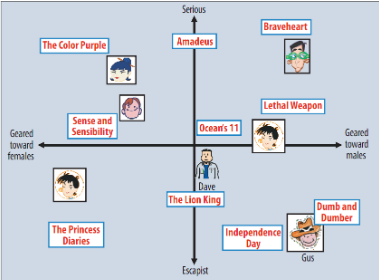
\includegraphics[width = 7cm]{graphic_representation.png}
\caption{Représentation Graphique des films rapport à certaines dimension}
\label{fig:representation_graphique}
\end{figure}

\section{Techniques de Décomposition Matricielle}
Plusieurs techniques sont déjà disponible pour la décomposition de matrice. Normalement, on factorise à partir des vecteurs propres de $MM^T$ ce qui entraînem l'orthogonalité. (analyse en composante principales \textbf{PCA}). On peut résumer le principe comme:\\

\centering
$M_{mxn} = Q_{mxl} P^T_{lxn}$\\
\justify

Ou m et n sont nos dimensions, l est le nombre de dimensions latente que nous souhaitons utiliser pour faire notre décomposition. Cette factorisation produit une matrice dense, de laquelle des calculs de similarités comme faite auparavant peuvent être utiliser pour faire des recommandations. Cette factorisation représente le produit Q et P et consitue une estimation (prédiction) de nos votes M.\\

Maintenant, supposons une matrice de votes utilisateurs-items M, il s'agit alors de la factoriser en 2+ matrice Q et P:\\

\centering
$M = QP^T$\\
\justify

Cette approche permet d'identifier des facteurs latents, qui sont en fait les dimensions sur laquelle nous allons décomposer nos matrices. Les facteurs se combinent linéairement pour augmenter et diminuer le vote (sommation). Dans ce calcule, Q représente la préférence des utilisateurs pour les facteurs et P représente l'appartenance des items aux facteurs. Cette méthode à donné les meilleurs résultats pour le prix Netflix en 2009. Il y a beaucoup de manière de créer les matrices Q et P.Comme par exemple la SVD ou la Décomposition en valeurs positive. Il existe plusieurs différents algorithme qui peuvent converger vers une solution.
\section{SVD}
Cette méthode est déjà bien connue en recherche d'information. Cette méthode se décompose de la façon suivant:\\

\centering
$M = U\Sigma V^T$\\
\justify

ou:
\begin{itemize}
\item U: matrice orthonormale qui représente les vecteurs propres de $MM^T$
\item V: matrice orthonormale qui représente les vecteurs propres de $M^TM$
\item $\Sigma$ : matrice diagonale qui représente les valeurs singulières de M (les racines des valeurs propres des vecteurs propres de $MM^T$ et $M^TM$
\end{itemize}

Les valeurs singulières de $\Sigma$sont ordonnées et indique l'amplitude relative de chaque vecteur propre. On utilise normalement les n premières valeurs singulières de  $\Sigma$ pour effectuer une réduction de dimensions ou n représente les facteurs latents. C'est ce qu'on nomme la \textbf{LSA} ou  Latent Semantic Analysis. Voici une exemple un peu plus graphique de la décomposition SVD:\\

\begin{figure}[!ht]
\centering
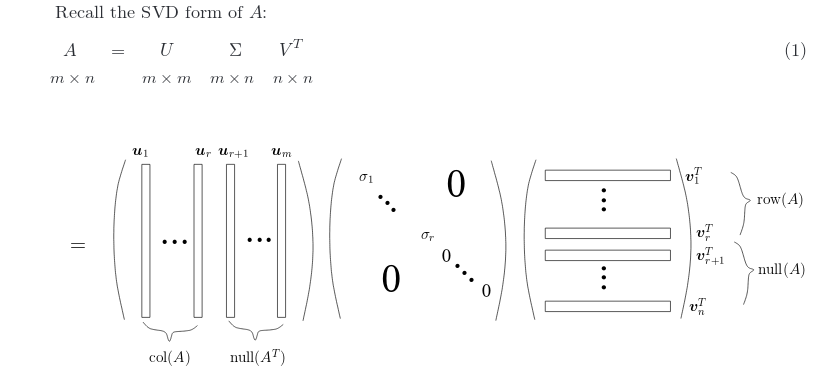
\includegraphics[width = \linewidth]{SVD.png}
\caption{Exemple visuel de la décomposition SVD}
\label{fig:SVD}
\end{figure}




\paragraph{Exemple dans le domaine de la RI}
Le domaine de la recherche d'information partage plusieurs techniques avec les systèmes de recommandations (en fait, ces technique sont directement utilisable pour les approches contenus). La matrice de recherche d'information à normalement une allure comme suit:\\

\begin{figure}[!ht]
\centering
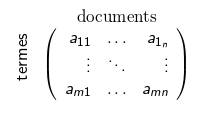
\includegraphics[width = 3cm]{recherche_information.png}
\caption{allure d'une matrice de recherche d'information}
\label{fig:recherche_information}
\end{figure}

\begin{figure}[!ht]
\centering
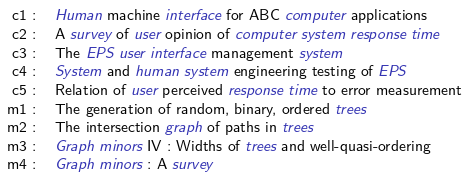
\includegraphics[width = 4cm]{exemple_contenu.png}
\caption{Exemple de contenue}
\label{fig:exemple_contenue}
\end{figure}

\begin{figure}[!ht]
\centering
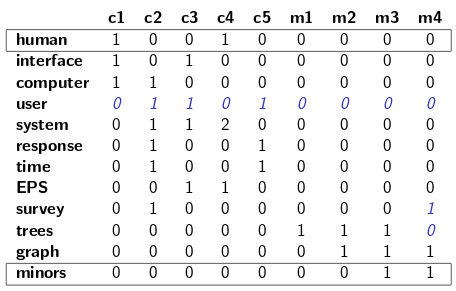
\includegraphics[width = 4cm]{matrice_terme.png}
\caption{Exemple de Matrice de termes}
\label{fig:exemple de matrice termes}
\end{figure}

Initialement, notre corrélations initiales des paires de terme était de -0.38 pour human-user ainsi que -0.29 pour human-minors. C'est mot veulent dirent presque la même chose, mais vu qu'il y a beaucoup de valeurs manquante la corrélation ne se fait pas bien. Par contre, en réduisant la dimensions, on ne conserve que les deux premières valeurs singulières (sachant qu'il n'y a que deux sources de documents). La matrice originale est reproduite avec les dimensions réduites à 2, alors toutes les valeurs singulières de la matrice diagonale $\Sigma$ sont mise à 0. \\

Après avoir réduit la dimension, nos corrélations pour les deux paires sont -0.94 ainsi que -0.83, ce qui est beaucoup mieux et représentent bien les attentes qu'on à des mots.\\

Pour résumer, la réduction de dimensions nous permet d'assigner des valeurs sur une échelle continue la ou il n'y avait pas de valeurs. Elle offre donc une solution au problème des matrices creuse. Et parfois, elle assigne des valeurs très justes des appartenances des variables aux facteurs latents comme l'exemple de Landauer et al. le démontre.

\section{Factorisation en Valeur non-négative + Valeurs manquantes}
D'autres méthodes sont disponible pour faire la décomposition de matrice. Une des autres méthodes très connus est la factorisation en valeurs non-négatives. elle va comme suit:\\

\centering
$R_{u * i} = W_{u * l} H_{l * i}$\\
\justify

On fait une factorisation en deux matrices ou l représente les facteurs latents. On applique une contrainte de valeurs non-négatives. Dans certains contexte, les valeurs négatives ne sont pas naturelles. Cette approche nous permet d'avoir des solutions multiples.\\

Normalement, pour trouver W et H on se sert d'une recherche par gradient (descente de gradient). Cette approche est non-déterministe alors sa peut prendre quand même longtemps converger. Par contre, on doit spécifier le nombre de dimension latentes k sur laquelles nous allons construire les matrices.\\

Pour l'ensemble des votes communs, k , on cherche les valeurs de W et H qui minimised l'équations suivantes:\\

\centering
$min_{p,q} \sum\limits_{(u,i)\in k} (r_{ui} - h_i^T w_u)^2 + \lambda(\parallel h_i \parallel^2 + \parallel w_u \parallel^2)$\\
\justify

ou le facteur avec le lambda est le facteur de régularisation qui limite les valeurs de p et q et que l'on contrôle par $\lambda$.
  
\section{Biais}
Une proportion importante de la variance des votes s'explique par:\\

\begin{itemize}
\item le biais utilisateur: la propention d'un individu à des votes faibles ou fort
\item le biais item: la popularité ou l'impopularité d'un item
\end{itemize}

Il faut donc inclure ces termes dans l'équation objective:\\

\centering
$r_{ui} = \mu + b_i + b_u + h_i^T q_u$\\
\justify

On peut ajouter beaucoup d'autres choses à l'équation, comme par exemple:\\

\begin{itemize}
\item Votes implicites (traces d'utilisateurs)
\item Facteurs Démographique
\end{itemize}
Certains termes sont en fonction du temps.. comme par exemple les biais qui peuvent changer avec le temps. Ou par exemple un vote qui peut avoir plus d'importance (TF-IDF???).\\

typiquement, les matrices de votes sont creuse. On peut proposer deux solution:\\
\begin{itemize}
\item Optimiser l'erreur quadratique avec la descente de gradient
\item Estimer les valeurs manquantes afin de créer une matrice dense.
\end{itemize}

\chapter{Modèle de Connaissance de l'utilisateur}
Comme on a vue dans l'intro, trois types d'information sont nécessaires pour une bonne modèlisation/personnalisation d'un système de recommandations, soit:\\

\begin{itemize}
\item \textbf{Intérêts}: On les retrouves plus ou moins implicitement dans les modèles de filtres d'informations. Les préférences, les votes, les comportements constituent en fait, d'un modèle utilisateur
\item \textbf{Connaissances}: très important pour les systèmes d'aide, les guide d'apprentissage et les systèmes tuteurs
\item \textbf{Buts}: Dans une certaines mesures, les intentions et les buts recherchés par l'utilisateur constituent aussi un modèle utilisateur, mais il est très dynamique, Il peut varier d'un instant à l'autre. On le verra avec les travaux sur la reconnaissance de plans. 
\end{itemize}

Dans cette section, on se concentrera beaucoup plus sur les modèles de la connaissances.\\

Les modèles de connaissances d'un utilisateurs sont très important dans plusieurs sorte de système de recommandations, soit:\\

\begin{itemize}
\item Guide d'étude: indique les matières sur lesquelles concentrer les efforts en vue d'un examen ou dans le cadre d'un cours. 
\item Tuteur: fournit un encadrement intelligent de matériel et exercices adaptés au réussites/échecs d'un étudiant
\item Exerciseur: adapte la difficulté des exercices/items au niveau de l'apprenant
\end{itemize}

Par exemple, on avait un système à la poly qui s'appelait Agata Z050, ce système évaluait les compétences en mathématiques des appliquants à la Polytechnique.\\

On peut modéliser la connaissance de plusieurs différentes façon:\\
\begin{itemize}
\item \textbf{Stéréotypes}: l'utilisateur est classifié selon un stéréotype, une classe comme expert, novice, intermdiate.. Ce modèle à l'avantage de la simplicité et peut facilement être entraîné avec des méthodes probabiliste.
\item \textbf{Hiérarchique} : Les connaissances sont organisées sous la forme d'une hiérarchie. La connaissance d'un noeud dépend de la connaissance de ses enfants.
\item \textbf{Par item}: Seuls des items observables sont utilisés pour modéliser la connaissances. De ces items, on peut déduire la connaissances de concepts non observable.
\end{itemize}

On peut aussi distinguer chaque modèle selon s'il comporte des paramêtres latents ou observables. et qu'ils sont construits par l'ingénierie de la connaissance ou par l'apprentissage automatique.\\

On peut utiliser d'autre dimensions à ce calcul, comme par exemple on peut utilisé des habiletés latentes ou observables. Les concepts sont des habiletés latentes car ils ne sont jamais directement observés (genre trigo vs calcul intégrale) mais plutôt induits à partir d'indices observables comme les réponse à des questions (items de tests).\\

On fait l'estimation des paramêtres par apprentissage par ingénierie. L'estimation des paramêtres par apprentissage avec des données empiriques permet l'automatisation et évite la subjectivité d'un modèle dont les paramêtres sont déterminés par un expert du domaine.\\

\begin{figure}[!ht]
\centering
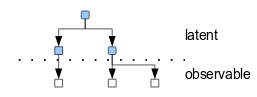
\includegraphics[width = 7cm]{latent_observable.png}
\caption{Comparaison graphique des facteurs latents vs. Observables.}
\label{fig:latent_observable}
\end{figure}

Les concepts, dans le cadre d'un apprentissage plus scolaires. sont des paramêtres latents puisqu'il ne sont jamais (??). Dans la représentation graphique de la fig\ref{fig:latent_observable}, les noeuds latents sont des concepts dans une structure hiéarachique dont les noeuds terminaux sont les items observables. (question/items). Pour résumer, les questions ont une appartenant à un certain concepts qu'on essaie de mesurer.
\section{Factorisation des matrices}
Normalement, on essaie de factoriser les matrices pour que les dimensions latentes représentent les différents sujets dans notre systèmes de recommandations et qu'on essaie de projeter nos questions comme ayant des composantes de nos différents sujet. Mais comment feront nous pour nous assurer quels items se rapportent à quel compétences/sujets??\\

On peut représenter nos questins comme étant une combinaisons de différents sujets. On appelle ce terme Q-matrix (q-matrice). Chaque question est représenter comme un coéfficient (un pourcentage?) qui représentent chaque rapport à la question au différents sujet qu'on essaient de modéliser.\\

\begin{figure}
\centering
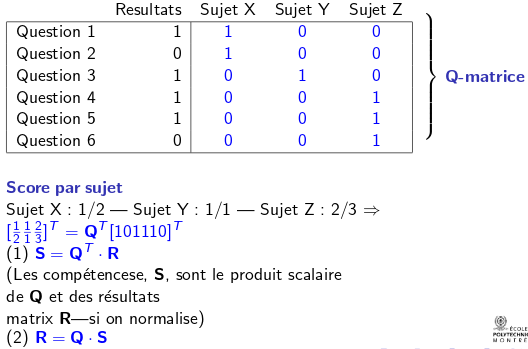
\includegraphics[width = 7cm]{q_matrix.png}
\caption{Exemple d'une Q-matrix}
\label{fig:q_matrix}
\end{figure}

On peut ajouter différentes variantes à la q-matrix:
\begin{itemize}
\item Elle peut avoir une à \textbf{plusieurs compétences par items} (un item comportant 50\% trigo, 40\% combinatoire ainsi que 10\% calcul intégrale..
\item On peut utiliser un \textbf{modèle conjonctifs}, c'est à dire que toutes les compétences sont nécessaires au succès (un mélange??)
\item un modèle \textbf{disjonctif}, ou une seule compétence amène au succès.
\item un modèle \textbf{compensatoire}, ou chaque compétences contribue linéairement aux chances de succès.
\end{itemize}

Ce sujet est très actif en recherche et soulève plusieurs questions:
\begin{itemize}
\item Le modèle linéaire est-il appropriés ? ESt-ce qu'on peut bien modéliser les compétences d'un individu avec une comparaison/combinaison linéaire des scores?
\item Un modèle conjonctif est-il plus performant ? Est-ce que sa prend vraiment une combinaison de toutes les sujets pour bien performer??

\item Les prédictions sont-elles meilleurs ou non aux autres modèles ? Comparaison entre les différents modèles ?
\end{itemize}

La factorisation de matrice peut amener une meilleur performance prédictive, mais pas nécessairement se prêter à l'interprétation.
\section{Utilisation d'un Modèle Bayésien}
On peut aussi utiliser des éléments observables comme évidence pour l'appartenance à une classe donnée. Posons comme exemple trois items, $X_1, X_2, X_3$ pouvant être soit réussi (X=1) ou échoué (X=0).Posons aussi deux stéréotypes, maître ou apprenti que nous exprimons comme étant respectivement $\theta$ = 1 ou $\theta$ = 0. Le modèle bayésien consiste à évaluer:\\

\centering
$P(\theta | X_1 = x_1, X_2 = x_2, X_3 = x_3)$
\justify

ou $x_i$ représente le succès ou l'échec à l'item correspondant. On abrège généralement l'expression précédente par :\\

\centering
$P(\theta | X_1, X_2, X_3)$
\justify

Maintenant, on peut poser comme énoncé que nos trois questions ($X_i$) sont des événements binomiales, c-à-d. qu'ils peuvent prendre des valeurs soit de 1 ou de 0 étant donné une réussite ou un échec respectivement. On peut représenter la probabilité d'appartenire à une classe (maitre = 1, apprenti = 0) en fonction de la fréquences $f$ d'occurence des classes comparé aux résultats obtenus dans les trois différentes questions, qui sont toutes les différentes combinaisons binomiales des résultats de questions. Avec la \textbf{correction de Laplace}, on peut calculer la probabilité d'appartenir à une classe $\theta_j$ avec la formule suivante:\\

\centering
$P(\theta_j) = \frac{f(\theta_j = 1) + 1}{(\sum\limits_v f(\theta_j = v)) + 2}$
\justify

en utilisant le tableau ci-haut, on peut dériver la probabilité d'appartenir à la classe $\theta = 1$ pour quelqu'un ayant eu une bonne réponse seulement qu'à la question 2:\\

\centering
$P(\theta_3) = P(\theta | X_1 = 0, X_2 = 1, X_3 = 0) = \frac{8 + 1}{25 + 8 + 2} = 0.26$\\

\justify


\subsection{Problèmes Combinatoire}
Par contre, cette méthode peut devenir beaucoup plus compliqués à mesure que sa avance. Dans notre exemple, nous avions trois question et deux classes... Pour un exemple plus réaliste ayant 10 questions, sa nous donne environ $2^10$ lignes (1024 entrées différentes) à calibrer et il nous faudrait des dizaines de milliers d'utilisateurs pour avoir une exemple pour chacun de ses différents cas, ce qui peut être quand même difficile... Il devient donc rapidement impossible de calibrer les probabilités conditionnelles. 


\section{Modèles d'espaces (sous-ensembles)}

n'est pas à l'examen.. voir slides
\subsection{Inférence et choix de Question}
n'est pas à l'examen.. voir slides
\section{Autres Modèles}
Pour répondre à ce problème, certains autres modèles peuvent être utiliser pour rendre les choses beaucoup moins compliquer:\\

\begin{itemize}
\item Modèls de réseaux de Bayes: On peut aussi modéliser les liens entre concepts eux-mêmes et entre les concepts et les items par différentes simplifications comme les 'noisy OR-gates' ou tout autre structure probabiliste qui a une signification:
\begin{figure}[!ht]
\centering
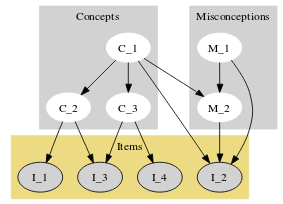
\includegraphics[width = 3cm]{bayes_network_knowledge.png}
\caption{Exemple d'un réseaux de Bayes pour modéliser la connaissance}
\label{fig:bayes_knowledge}
\end{figure}

\item Modèles à base de règles: Un autre modèle qui utilise des règles our établire des diagnostics précis et analyser des comportements plus complexes. Il peut être combinés à un modèle probabiliste.
\item Modèles simple: Finalement, on peut aussi utiliser une matrice et une simple formule de sommation pour indiquer le niveau de maîtrise de différents concepts à l'instar d'un examen.
\end{itemize}

Les modèles graphiques bayésiens sont très répandus dans le domaine de la modélisation des connaissances des apprenants. Ils sont particulièrement utilisé pour modéliser les concepts entres eux et leur relations. Vous pouvez voir à la fig \ref{fig:bayes_knowledge} un exemple d'un réseaux qui modélise des questions en fonction des concepts et des méconceptions classique.\\

Avec les réseaux bayésiens, on peut faire de l'inférence. Certaines structure comme les arbres se prête â un calcul exact. Des structure libres doivent recourir à des algorithmes d'expectation-maximisation (EM) ou plus communément, maximum-likelihood. Ce qui peut être très couteux.\\

ces algorithmes peuvent prendre plusieurs formes. voici certaines formes communes avec les grandes lignes:

\begin{itemize}
\item En commençant par les racines, on assigne des valeurs aléatoire mais selon les probabilités initiales
\item On propages les assignations vers les noeuds enfants en respectant les valeurs assignées aux noeuds parents.
\item On créé ainsi plusieurs échantillons à partir desquels on recalcule les probabilités conditionnelles à partir des assignations aléatoires.
\item Les nouvelles probablités sont réutilisées pour créer de nouveaux échantillons.
\end{itemize}

Souvent, on utilise un modèle \textit{ad hoc} qui simplifie les calculs mais ne respecte pa sla sémantique des inférences bayésiennes.
\section{Régression Logistique}
Présumons que le succès d'un individu à répondre correctement à une série de question $(X_1,X_2, X_3...,X_n)$ dépend de son habileté, $\theta$ qui serait un nombre continue dans le spectre réel. La probabilité d'observer une série spécifique de réponse, $(x_1, x_2,x_3,...,x_n)$ est donc:\\

\centering
$P(x1,x_2,...x_n|\theta) = \prod\limits_i P(x_i|\theta)$
\justify

Le problème consiste donc à trouver la valeur de $\theta$ qui maximisera cette probabilité. Il nous faut un modèle de $P(X_i|\theta)$ comme celui de la figure ci-contre, qui correspond à la figure ci-dessous, qui est en fait la \textbf{fonction sigmoïde}:\\

\centering
$P(X_i|\theta) = \frac{1}{1 + e^{-\theta}}$
\justify

\begin{figure}[!ht]
\centering
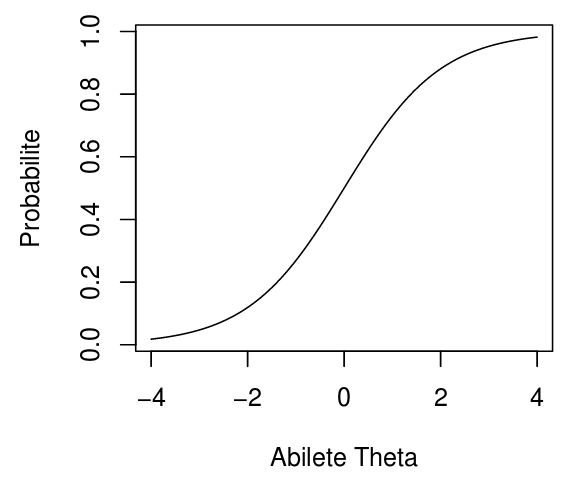
\includegraphics[width = 5cm]{sigmoide.png}
\caption{Allure de la fonction sigmoide}
\label{fig:sigmoide}
\end{figure}

Prenons comme exemple un individu qui obtient ces réponse pour 7 questions étant totalement indépendantes:\\

\centering
(0,1,1,0,0,0,0)
\justify

La probabilité d'observer cette séquence s'il avait une habileté $\theta = 1$ serait proportionelle à :\\

\centering
$P(X_i = 1| \theta = 1) = \frac{1}{1 + e^{-1}} = 0.731$\\

donc, pour deux évenement qui sont égale à 1 et 5 autres qui sont égale à 0...\\

$0.731^2 * (1 - 0.731)^5 = 0.001$\\
\justify

Sont les chances qu'un individu obtiennent ces résultats étant donné son habileté $\theta = 1$. On peut recommencer l'expérience avec un différent $\theta = -1$ qui nous donnerait une probabilité de 0.015. on peut faire un graphique avec les différentes valeurs de theta possible et prendre le maximum comme étant l'habileté la plus probable pour notre individu.\\

\begin{figure}[!ht]
\centering
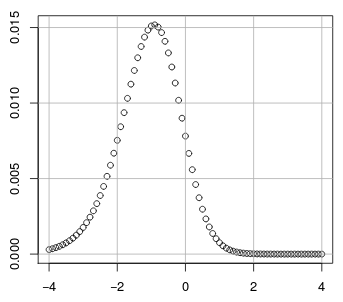
\includegraphics[width = 6cm]{graph_theta.png}
\caption{Habiletés différentes pour notre individus}
\label{fig:graph_theta}
\end{figure} 

\subsection{Modèles TRI}
Le modèle le plus répandus pour modéliser les réponses à des items d'un test est celui de la Théorie des Réponses aux Items, abrégés \textbf{TRI}. Ce modèle s'inspire de la fonction sigmoïde mais il comprend deux paramètres supplémentaires:
\begin{itemize}
\item a : la discrimination d'un item qui détermine la pente de notre fonction sigmoïde.
\item b : la difficulté d'un item qui détermine l'absisse
\end{itemize}

La fonction résultante est celle de la réponse caractéristique à un item (Item characteristic Curve - ICC):\\

\centering
$P(X_i|\theta) = \frac{1}{1 + e^{-a_i(\theta - b_i}}$
\justify

Ces fonctions donne comme résultats finaux:\\

\begin{figure}[!ht]
\centering
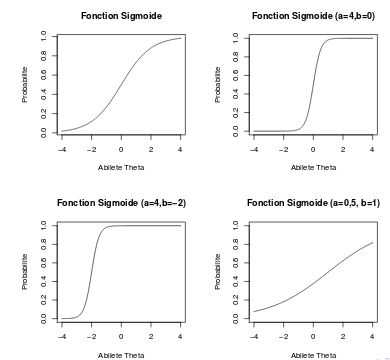
\includegraphics[width = 7cm]{tri.png}
\caption{Différentes fonctions TRI}
\label{fig:tri}
\end{figure}

\chapter{Articles}

\section{Deconstructing Recommender Systems}
 One morning in April, we each directed our browsers to Amazon.com’s website. Not only did the site greet us by name, the home page opened with a host of suggested purchases. It directed Joe to Barry Greenstein’s Ace on the River: An Advanced Poker Guide, Jonah Lehrer’s Imagine: How Creativity Works, and Michael Lewis’s Boomerang: Travels in the New Third World. For John it selected Dave Barry’s Only Travel Guide You’ll Ever Need, the spy novel Mission to Paris, by Alan Furst, and the banking exposé The Big Short: Inside the Doomsday Machine, also by Michael Lewis.\\

By now, online shoppers are accustomed to getting these personalized suggestions. Netflix suggests videos to watch. TiVo records programs on its own, just in case we’re interested. And Pandora builds personalized music streams by predicting what we’ll want to listen to.\\

All of these suggestions come from recommender systems. Driven by computer algorithms, recommenders help consumers by selecting products they will probably like and might buy based on their browsing, searches, purchases, and preferences. Designed to help retailers boost sales, recommenders are a huge and growing business. Meanwhile, the field of recommender system development has grown from a couple of dozen researchers in the mid-1990s to hundreds of researchers today—working for universities, the large online retailers, and dozens of other companies whose sole focus is on these types of systems.\\

Over the years, recommenders have evolved considerably. They started as relatively crude and often inaccurate predictors of behavior. But the systems improved quickly as more and different types of data about website users became available and they were able to apply innovative algorithms to that data. Today, recommenders are extremely sophisticated and specialized systems that often seem to know you better than you know yourself. And they’re expanding beyond retail sites. Universities use them to steer students to courses. Cellphone companies rely on them to predict which users are in danger of switching to another provider. And conference organizers have tested them for assigning papers to peer reviewers.\\

The two of us have been building and studying recommender systems since their early days, initially as academic researchers working on the GroupLens Project. Begun in 1992, GroupLens sorted through messages in Usenet discussion forums and pointed users to threads they might be interested in but had not yet discovered on their own. Several years later, we founded Net Perceptions, the leading recommender company during the first Internet boom. Our experience, therefore, gives us a lot of insight into what’s going on behind the scenes at Amazon and other online retailers, even though those companies seldom speak publicly about exactly how their recommendations work. (In this article, our analysis is based on educated observation and deduction, not on any inside information.) Here’s what we know.\\


https://spectrum.ieee.org/computing/software/deconstructing-recommender-systems

\section{Content-Boosted Collaborative Filtering for Improved Recommendations}
\paragraph{Abstract}
Most  recommender  systems  use  Collaborative  Filtering  or
Content-based  methods  to predict  new  items of interest for
a user.  While both methods have their own advantages, indi-
vidually they fail to provide good recommendations in many
situations.  Incorporating components from both methods, a
hybrid recommender system can overcome these shortcom-
ings. In this paper, we present an elegant and effective frame-
work for combining content and collaboration. Our approach
uses a content-based predictor to enhance existing user data,
and then provides  personalized  suggestions  through  collab-
orative filtering.  We present experimental results that show
how this approach,
Content-Boosted Collaborative Filtering
,
performs better than a pure content-based predictor, pure col-
laborative filter, and a naive hybrid approach.

\paragraph{Conclusion}

Incorporating content information into collaborative filter-
ing can significantly improve predictions of a recommender
system.   In this paper, we have provided an effective way
of  achieving  this.   We  have  shown  how  Content-boosted
Collaborative Filtering performs better than a pure content-
based predictor, collaborative filtering, and a naive hybrid of
the two.
CBCF  elegantly  exploits  content  within  a  collaborative
framework. It overcomes the disadvantages of both collabo-
rative filtering and content-based methods, by bolstering CF
with content and vice versa. Further, due to the modular na-
ture of our framework, any improvements in collaborative
filtering or content-based recommending can be easily ex-
ploited to build a more powerful system.
Although
CBCF  performs  consistently  better  than  pure
CF,  the  difference in  performance is  not  very  large (
4
\%).
The performance of our system can be boosted by using the
methods described earlier.  Experiments comparing the dif-
ferent approaches of combining content and collaboration,
outlined in the previous section, are also needed.

\section{On the recommending of citations for research papers}
\paragraph{Abstract}
Collaborative filtering has proven to be valuable for recommending items in many different domains. In this paper, we explore the use of collaborative filtering to recommend research papers, using the citation web between papers to create the ratings matrix. Specifically, we tested the ability of collaborative filtering to recommend citations that would be suitable additional references for a target research paper. We investigated six algorithms for selecting citations, evaluating them through offline experiments against a database of over 186,000 research papers contained in ResearchIndex. We also performed an online experiment with over 120 users to gauge user opinion of the effectiveness of the algorithms and of the utility of such recommendations for common research tasks. We found large differences in the accuracy of the algorithms in the offline experiment, especially when balanced for coverage. In the online experiment, users felt they received quality recommendations, and were enthusiastic about the idea of receiving recommendations in this domain.
\section{Bringing PageRank to the citation analysis}
\paragraph{Abstract}
The paper attempts to provide an alternative method for measuring the importance of scientific papers based on the Google’s PageRank. The method is a meaningful extension of the common integer counting of citations and is then experimented for bringing PageRank to the citation analysis in a large citation network. It offers a more integrated picture of the publications’ influence in a specific field. We firstly calculate the PageRanks of scientific papers. The distributional characteristics and comparison with the traditionally used number of citations are then analyzed in detail. Furthermore, the PageRank is implemented in the evaluation of research influence for several countries in the field of Biochemistry and Molecular Biology during the time period of 2000–2005. Finally, some advantages of bringing PageRank to the citation analysis are concluded.
\section{The YouTube video recommendation system}
\paragraph{Abstract}
We discuss the video recommendation system in use at YouTube, the world's most popular online video community. The system recommends personalized sets of videos to users based on their activity on the site. We discuss some of the unique challenges that the system faces and how we address them. In addition, we provide details on the experimentation and evaluation framework used to test and tune new algorithms. We also present some of the findings from these experiments.
\section{Matrix Factorization for Recommender Systems}
??
\section{Deep Neural Networks for YouTube Recommendations}
\paragraph{Abstract}
YouTube represents one of the largest scale and most sophisticated industrial recommendation systems in existence. In this paper, we describe the system at a high level and focus on the dramatic performance improvements brought by deep learning. The paper is split according to the classic two-stage information retrieval dichotomy: first, we detail a deep candidate generation model and then describe a separate deep ranking model. We also provide practical lessons and insights derived from designing, iterating and maintaining a massive recommendation system with enormous user-facing impact. 
\section{Multicriteria User Modeling in Recommender Systems}
\paragraph{Abstract}
The paper mentions that a hybrid recommender systems framework creates user-profile groups before applying a collaborative-filtering algorithm by incorporating techniques from the multiple-criteria decision-analysis (MCDA) field.
\section{Recommendation Systems for Software Engineering}
\paragraph{Abstract}
Software development can be challenging because of the large information spaces that developers must navigate. Without assistance, developers can become bogged down and spend a disproportionate amount of their time seeking information at the expense of other value-producing tasks. Recommendation systems for software engineering (RSSEs) are software tools that can assist developers with a wide range of activities, from reusing code to writing effective bug reports. The authors provide an overview of recommendation systems for software engineering: what they are, what they can do for developers, and what they might do in the future.
\section{An energy efficient mobile recommender systems}
??
\section{AutoRec : Autoencoder meet Collaborative Filtering}
\paragraph{Abstract}
This paper proposes AutoRec, a novel autoencoder frame-
work for collaborative filtering (CF). Empirically, AutoRec’s
compact and efficiently trainable model outperforms state-
of-the-art CF techniques (biased matrix factorization, RBM-
CF and LLORMA) on the Movielens and Netflix datasets.
\section{Collaborative Filtering with Stacked Denoising AutoEncoders and Sparse Inputs}
\paragraph{Abstract}
Neural networks have not been widely studied in Collaborative Filtering.
For instance, no paper using neural networks was published during the Net-
flix Prize apart from Salakhutdinov et al’s work on Restricted Boltzmann
Machine (RBM) [14].  While deep learning has tremendous success in image
and speech recognition, sparse inputs received less attention and remains
a challenging problem for neural networks.  Nonetheless, sparse inputs are
critical for collaborative filtering.  In this paper, we introduce a neural net-
work architecture which computes a non-linear matrix factorization from
sparse rating inputs.  We show experimentally on the movieLens and jester
dataset that our method performs as well as the best collaborative filtering
algorithms.  We provide an implementation of the algorithm as a reusable
plugin for Torch [4], a popular neural network framework
\section{Predicting User Tasks : I know what you are doing}
??
\section{Fewer Clicks and Less Frustration: Reducing the Cost of Reaching the Right Folder }
\paragraph{Abstract}
Helping computer users rapidly locate files in their folder hierarchies has become an important research topic in today's intelligent user interface design. This paper reports on FolderPredictor, a software system that can reduce the cost of locating files in hierarchical folders. FolderPredictor applies a cost-sensitive prediction algorithm to the user's previous file access information to predict the next folder that will be accessed. Experimental results show that, on average, FolderPredictor reduces the cost of locating a file by 50\%. Another advantage of FolderPredictor is that it does not require users to adapt to a new interface, but rather meshes with the existing interface for opening files on the Windows platform.
\section{User-Based Collaborative-Filtering Recommendation Algorithms on Hadoop}
\paragraph{Abstract}
Collaborative Filtering(CF) algorithms are widely used in a lot of recommender systems, however, the computational complexity of CF is high thus hinder their use in large scale systems. In this paper, we implement user-based CF algorithm on a cloud computing platform, namely Hadoop, to solve the scalability problem of CF. Experimental results show that a simple method that partition users into groups according to two basic principles, i.e., tidy arrangement of mapper number to overcome the initiation of mapper and partition task equally such that all processors finish task at the same time, can achieve linear speedup
\section{Scaling-Up Item-Based Collaborative Filtering Recommendation Algorithm Based on Hadoop}
\paragraph{Abstract}
Collaborative filtering (CF) techniques have achieved widespread success in E-commerce nowadays. The tremendous growth of the number of customers and products in recent years poses some key challenges for recommender systems in which high quality recommendations are required and more recommendations per second for millions of customers and products need to be performed. Thus, the improvement of scalability and efficiency of collaborative filtering (CF) algorithms become increasingly important and difficult. In this paper, we developed and implemented a scaling-up item-based collaborative filtering algorithm on MapReduce, by splitting the three most costly computations in the proposed algorithm into four Map-Reduce phases, each of which can be independently executed on different nodes in parallel. We also proposed efficient partition strategies not only to enable the parallel computation in each Map-Reduce phase but also to maximize data locality to minimize the communication cost. Experimental results effectively showed the good performance in scalability and efficiency of the item-based CF algorithm on a Hadoop cluster.
\section{Benefits and costs of adaptive user interfaces}
\paragraph{Abstract}
The paper examines the positive and the possible adverse effects of adaptive user interfaces (AUIs) in the context of an in-vehicle
telematic system as a function of four factors: (1) four different levels of adaptivity (ranging from manual to fully adaptive with
intermediate levels); (2) different tasks; (3) routine (familiar) and non-routine (unfamiliar) situations; and (4) different user age groups.
Both experiments included three sessions during which participants drove a simple driving simulator and performed tasks with the
telematic system at one of the adaptivity levels. We measured task performance times and lane position variance. Adaptivity was not
always equally beneficial, and its benefits depended on a number of factors, including the frequency in which the tasks were performed,
the user’s age, the difficulty of the task and the user’s involvement in the task. In familiar, routine situations, a fully adaptive system was
beneficial for all participants, particularly older ones. In unfamiliar situations, to which the AUI was not adjusted, cognitive workload
increased substantially, adversely affecting performance. Intermediate levels of adaptivity keep users involved in the task and help them
become more proficient when performing both routine and non-routine tasks. However, intermediate levels of adaptivity should also be
implemented with care, because they may also have adverse effects when users encounter non-routine situations.


\section{Being Accurate is Not Enough: How Accuracy Metrics have hurt Recommender Systems }
\paragraph{Abstract}
Recommender systems have shown great potential to 
help users find interesting and relevant items from 
within a large information space.  Most research up to 
this point has focused on improving the accuracy of 
recommender systems.  We be
lieve that not only has 
this narrow focus been misguided, but has even been 
detrimental to the field.  The recommendations that are 
most accurate according to the standard metrics are 
sometimes not the recommendations that are most 
useful to users. In this paper, we propose informal 
arguments that the recommender community should 
move beyond the conventional accuracy metrics and 
their associated experimental methodologies.  We 
propose new user-centric directions for evaluating 
recommender systems
\section{The Impact of YouTube Recommendation System on Video Views}
\paragraph{Abstract}
Hosting a collection of millions of videos, YouTube offers
several features to help users discover the videos of their in-
terest. For example, YouTube provides video search, related
video recommendation and front page highlight. The under-
standing of how these features drive video views is useful for
creating a strategy to drive video popularity.  In this pa-
per, we perform a measurement study on data sets crawled
from YouTube and find that the related video recommenda-
tion, which recommends the videos that are related to the
video a user is watching, is one of the most important view
sources of videos. Despite the fact that the YouTube video
search is the number one source of views in aggregation, the
related video recommendation is the main source of views
for the majority of the videos on YouTube. Furthermore,
our results reveal that there is a strong correlation between
the view count of a video and the average view count of its
top referrer videos. This implies that a video has a higher
chance to become popular when it is placed on the related
video recommendation lists of popular videos. We also find
that the click through rate from a video to its related videos
is high and the position of a video in a related video list
plays a critical role in the click through rate. Finally, our
evaluation of the impact of the related video recommenda-
tion system on the diversity of video views indicates that
the current recommendation system helps to increase the
diversity of video views in aggregation.

\section{LinkedVis: exploring social and semantic career recommendations}
\paragraph{Abstract}
This paper presents LinkedVis, an interactive visual recommender system that combines social and semantic knowledge to produce career recommendations based on the LinkedIn API. A collaborative (social) approach is employed to identify professionals with similar career paths and produce personalized recommendations of both companies and roles. To unify semantically identical but lexically distinct entities and arrive at better user models, we employ lightweight natural language processing and entity resolution using semantic information from a variety of end-points on the web. Elements from the underlying recommendation algorithm are exposed through an interactive interface that allows users to manipulate different aspects of the algorithm and the data it operates on, allowing users to explore a variety of "what-if" scenarios around their current profile. We evaluate LinkedVis through leave-one-out accuracy and diversity experiments on a data corpus collected from 47 users and their LinkedIn connections, as well as through a supervised study of 27 users exploring their own profile and recommendations interactively. Results show that our approach outperforms a benchmark recommendation algorithm without semantic resolution in terms of accuracy and diversity, and that the ability to tweak recommendations interactively by adjusting profile item and social connection weights further improves predictive accuracy. Questionnaires on the user experience with the explanatory and interactive aspects of the application reveal very high user acceptance and satisfaction.

\section{Recommender Systems – Beyond Matrix Completion}
\paragraph{Abstract}
The use of recommender systems has exploded over the
last decade, making personalized recommendations ubiqui-
tous online. Most of the major companies, including Google,
Facebook,  Twitter,  LinkedIn,  Netflix,  Amazon,  Microsoft,
Yahoo!,  eBay,  Pandora,  Spotify  and  many  others  use  rec-
ommender systems (RS) within their services.
These systems are used to recommend a whole range of
items, including consumer products, movies, songs, friends,
news articles, restaurants and various others.  Recommender
systems  constitute  a  mission-critical  technology  in  several
companies.  For example, Netflix reports that at least 75%
of  their  downloads  and  rentals  come  from  their  RS,  thus
making it of strategic importance to the company
1
.
In some ways, the systems that produce these recommen-
dations are remarkable.  They incorporate a variety of sig-
nals about characteristics of the users and items, including
people’s explicit or implicit evaluations of items.  The sys-
tems  process  these  signals  at  a  massive  scale,  often  under
real-time constraints.  Most importantly, the recommenda-
tions are of significant quality on average.  In empirical tests,
people choose the suggested items far more often than they
choose suggested items based on unpersonalized benchmark
algorithms such as overall popularity.
In other ways, the systems that produce these recommen-
dations are sometimes remarkably bad.  Occasionally, they make  recommendations  that  are  embarrassing  for  the  sys-
tem, such as recommending to a faculty member an intro-
ductory book from the “for dummies” series on a topic she is
expert in.  Or, they continue recommending items the user
is no longer interested in.  Shortcomings like these motivate
ongoing  research  both  in  industry  and  academia,  and  rec-
ommender systems are a very active field of research today.
To provide an understanding of the state-of-the-art of rec-
ommender systems, this article starts with a bit of history,
culminating  in  the  million-dollar  Netflix  challenge.   That
challenge led to a formulation of the recommendation prob-
lem  as  one  of  matrix  completion:  given  a  matrix  of  users
by items, with item ratings as cells, how well can an algo-
rithm predict the values in some cells that are deliberately
held out?  However, algorithms with maximum accuracy at
the  matrix  completion  task  are  not  sufficient  to  make  the
best recommendations in many practical settings.  We will
describe  why,  review  some  of  the  approaches  that  current
research  is  taking  to  do  better,  and  finally  sketch  ways  of
approaching the recommendation problem in a more com-
prehensive way in the future.
\section{A Graph-based Recommender System for Digital Library}
\paragraph{Abstract}
Research  shows  that  recommendations  comprise  a  valuable  
service for users of a digital library [11]. While most existing 
recommender   systems   rely   either   on   a   content-based   
approach     or     a     collaborative     approach     to     make     
recommendations,     there     is     potential     to     improve     
recommendation  quality  by  using  a  combination  of  both  
approaches (a hybrid approach). In this paper, we report how 
we  tested  the  idea  of  using  a  graph-based  recommender  
system   that   naturally   combines   the   content-based   and   
collaborative  approaches.  Due  to  the  similarity  between  our  
problem   and   a   concept   retrieval   task,   a   Hopfield   net   
algorithm  was  used  to  exploit  high-degree  book-book,  user-
user and book-user associations. Sample hold-out testing and 
preliminary  subject  testing  were  conducted  to  evaluate  the  
system,  by  which  it  was  found  that  the  system  gained  
improvement  with  respect  to  both  precision  and  recall  by  
combining   content-based   and   collaborative   approaches.   
However,   no   significant   improvement   was   observed   by   
exploiting high-degree associations. 
\section{Comparing context-aware recommender systems in terms of accuracy and diversity}
\paragraph{Abstract}
Although the area of context-aware recommender systems (CARS) has made a significant progress over the last several years, the problem of comparing various contextual pre-filtering, post-filtering and contextual modeling methods remained fairly unexplored. In this paper, we address this problem and compare several contextual pre-filtering, post-filtering and contextual modeling methods in terms of the accuracy and diversity of their recommendations to determine which methods outperform the others and under which circumstances. To this end, we consider three major factors affecting performance of CARS methods, such as the type of the recommendation task, context granularity and the type of the recommendation data. We show that none of the considered CARS methods uniformly dominates the others across all of these factors and other experimental settings; but that a certain group of contextual modeling methods constitutes a reliable “best bet” when choosing a sound CARS approach since they provide a good balance of accuracy and diversity of contextual recommendations.
\section{Collaborative Topic Modeling for Recommending Scientific Articles}
\paragraph{Abstract}
Researchers have access to large online archives of scientific arti-
cles. As a consequence, finding relevant papers has become more
difficult. Newly formed online communities of researchers sharing
citations provides a new way to solve this problem. In this paper, we
develop an algorithm to recommend scientific articles to users of an
online community. Our approach combines the merits of traditional
collaborative filtering and probabilistic topic modeling. It provides
an interpretable latent structure for users and items, and can form
recommendations about both existing and newly published articles.
We study a large subset of data from CiteULike, a bibliography shar-
ing service, and show that our algorithm provides a more effective
recommender system than traditional collaborative filtering

\end{document}